% Modelo de Dissertação em Latex para o PPG em Engenharia Mecânica da UERJ
% Este modelo foi adaptado da versão disponibilizada no site da Engenharia Elétrica da UERJ
% http://www.pel.uerj.br/publico/Modelo_LaTeX_Dissertacao_UERJ.rar
% http://www.pel.uerj.br/defesas/
%
% Utilizei o WinEdt 6.0 com Miktex 2.9
%
% Para gerar o PDF usei a opção PDFTeXfy com o documento [masterthesis.tex] aberto e em foco.
%
% Não consegui usar as figuras em EPS como o modelo original. Usei PNG e JPG sem problemas.
%
% Felipe M. - 20/06/2012
%
% 												Command             10pt    11pt    12pt
% 												\tiny               5       6       6
% 												\scriptsize         7       8       8
% 												\footnotesize       8       9       10
% 												\small              9       10      10.95
% 												\normalsize         10      10.95   12
% 												\large              12      12      14.4
% 												\Large              14.4    14.4    17.28
% 												\LARGE              17.28   17.28   20.74
% 												\huge               20.74   20.74   24.88
% 												\Huge               24.88   24.88   24.88


\documentclass[a4paper,12pt,oneside,openany]{uerj}
\usepackage[english,brazil]{babel}
% \usepackage[math]{iwona}
% \DeclareFontFamily{U}{futm}{}
% \DeclareFontShape{U}{futm}{m}{n}{
%   <-> fourier-bb % changed from .92 to 1
%   }{}
% \DeclareMathAlphabet{\mathbb}{U}{futm}{m}{n}
%\usepackage[latin1]{inputenc}
%\usepackage{fourier}
%\usepackage[utopia]{mathdesign}
%\usepackage{fouriernc}
%\usepackage{fontspec}
\usepackage{mathptmx} % Times New Roman

%\usepackage{Times}
% \usepackage[T1]{fontenc}
\usepackage{lmodern}
%\setmainfont{Times}
%\setmainfont{Arial}
\usepackage[utf8]{inputenc}
\usepackage{enumerate}
\usepackage{cite}
\usepackage{epsf,epsfig,psfig}
\usepackage{pagina}
\usepackage{indentfirst}
\usepackage{theorem}
\usepackage{fancyhdr}
\usepackage{setspace}
\usepackage{boxedminipage}
\usepackage{float}
%\usepackage[style=base]{caption}
\usepackage{subcaption}
%\captionsetup{compatibility=false}
%\usepackage{subcaption}
%\usepackage[caption=false]{subfig}
\usepackage{silence}
\WarningFilter{caption}{Unsupported document class}
\usepackage{makeidx}
\usepackage{amsmath}
\usepackage{mathtools}
\usepackage{geometry}
\usepackage[hidelinks]{hyperref}
\pdfstringdefDisableCommands{\let\uppercase\relax} % desabilitar alguns warnings e \uppercase

%------------------------------------------------
\usepackage{xargs}                      % Use more than one optional parameter in a new commands
\usepackage[pdftex,dvipsnames]{xcolor}  % Coloured text etc.
\usepackage[colorinlistoftodos,prependcaption,textsize=normalsize]{todonotes}
\newcommandx{\balao}[2][1=]{\todo[linecolor=red,backgroundcolor=red!25,bordercolor=red,#1]{#2}}
\newcommandx{\change}[2][1=]{\todo[linecolor=blue,backgroundcolor=blue!25,bordercolor=blue,#1]{#2}}
\newcommandx{\info}[2][1=]{\todo[linecolor=OliveGreen,backgroundcolor=OliveGreen!25,bordercolor=OliveGreen,#1]{#2}}
\newcommandx{\improvement}[2][1=]{\todo[linecolor=Plum,backgroundcolor=Plum!25,bordercolor=Plum,#1]{#2}}
\newcommandx{\thiswillnotshow}[2][1=]{\todo[disable,#1]{#2}}
\newcommandx{\authorName}{Lucas Carvalho de Sousa}
\newcommandx{\mainTitle}{Simulação Numérica De Escoamentos Dispersos Utilizando Método De Elementos Finitos}
\newcommandx{\curYear}{2019}
\newcommandx{\numPages}{xx f}
%------------------------------------------------
%------------------------------------------------
\usepackage{geometry}
\usepackage{mathtools}
%------------------------------------------------

\makeindex


\newtheorem{deff}{Definição}[section]
\numberwithin{equation}{chapter}

\theoremstyle{plain}

\bibliographystyle{abnt-num}



\begin{document}

% \hypersetup{
%      colorlinks,
%     citecolor=black,
%     filecolor=black,
%     linkcolor=black,
%     urlcolor=black,
%     linktoc=all
% }

\thispagestyle{empty}\begin{titlepage}
\begin{center}

	\vspace{-0.5cm}

  \begin{figure}[hbt!]
		\begin{flushleft}
		   
\includegraphics[scale=0.3]{./00_Pre_textuais/logo_uerj_pb.png}
		\end{flushleft}
	\end{figure}
	\vspace{-4cm}

  \hspace{2cm}\large{\textbf{Universidade do Estado do Rio de Janeiro}}\\
  \hspace{2cm}\large{Centro de Tecnologia e Ciências}\\
  \hspace{2cm}\large{Faculdade de Engenharia}\\

  \hspace{2cm}\large{}\\
  \hspace{2cm}\large{}\\
  \hspace{2cm}\large{}\\
  \hspace{2cm}\large{}\\

  \par
  {\large{\authorName}}

  \hspace{2cm}\large{}\\
  \hspace{2cm}\large{}\\
  \hspace{2cm}\large{}\\
  \hspace{2cm}\large{}\\


  \par
  {\large\textbf{\mainTitle}}%Título do Trabalho


  \par\vfill
  Rio de Janeiro\\ \curYear

\end{center}
\end{titlepage}
\pagebreak\thispagestyle{empty}\begin{center}

\authorName

% \vfill
\vspace{2cm}

\textbf{\mainTitle}

\vspace{1.0cm}

\begin{figure}[hbt!]
\begin{center}

\includegraphics[width=10.48cm,height=10.8cm]{./00_Pre_textuais/logo_uerj_gnd_pb.png}
\end{center}
\end{figure}

\vspace{-9cm}
\begin{flushright}
\parbox{8cm}{
\singlespacing{Projeto Final apresentado a Faculdade de Engenharia da Universidade do Estado do Rio de Janeiro, para obtenção do grau de bacharel em Engenharia Mecânica}.
}
% \singlespacing{Dissertação apresentada, como requisito\linebreak parcial para obtenção do título de Mestre em Ciências, ao Programa de Pós-Graduação em Engenharia Mecânica, da Universidade do Estado do Rio de Janeiro. Área de\linebreak concentração: Fenômenos de Transporte}.
% }
\end{flushright}

\vspace{4.0cm}

Orientador: Prof. D.Sc. Gustavo R. Anjos\\

\par\vfill
%\vspace{2cm}

Rio de Janeiro\\ \curYear

\end{center}
\pagebreak\thispagestyle{empty}% Depois de preparar seu trabalho, você deverá enviá-lo para a Biblioteca CTC/B para avaliação do formato e elaboração da Ficha catalográfica.
% Com a ficha pronta (fornecida pela Biblioteca), você poderá alterar este trecho do trabalho em definitivo.
%
% Para este processo, enviei a dissertação em PDF para o email: ctcb.uerj.bdtd@gmail.com (Tratei de todos os detlahes com a Sra. Márcia)
% Qualquer dúvida, veja os contatos da Biblioteca no site da Rede Sirius: http://www.rsirius.uerj.br/
% 


\begin{titlepage}
	\begin{center}
\vfill
\singlespacing
	\vspace*{75mm}
	{Ficha elaborada pelo autor através do\\ \vspace{1.5mm}
	 Sistema para Geração Automática de Ficha Catalográfica da Rede Sirius - UERJ}\\
	\vspace{1.5mm}
	\begin{boxedminipage}{140mm}
	\begin{minipage}{5mm}
		\vspace{-94mm}
		S725
	\end{minipage}
	\hfill
	\raisebox{8.5mm}{
	\begin{minipage}[top]{115mm}
		\vspace*{5mm}

		Sousa, Lucas Carvalho de\\
		\phantom{XX}\mainTitle\,/\,\authorName. -- 2019.\\
		\phantom{XX}\numPages.\\
		\phantom{XX}\\
		\phantom{XX}Orientador: Gustavo Rabello dos Anjos\\ \hspace*{5mm}
       		\phantom{XX}Trabalho de Conclusão de Curso apresentado à Universidade do Estado do Rio de Janeiro, Faculdade de Engenharia, para obtenção do grau de bacharel em Engenharia Mecânica.\\
		\phantom{XX}\\
		\phantom{XX}1. Método de Elementos Finitos - Monografias. 2. Formulação Corrente-Vorticidade - Monografias. 3. Escoamento Multifásico - Monografias. 4. Escoamento Particulado - Monografias. 5. Programação Orientada a Objetos - Monografias. I. Anjos, Gustavo Rabello dos. II. Universidade do Estado do Rio de Janeiro. Faculdade de Engenharia. III. Título.
	\end{minipage}}
	\vspace*{5mm}
	\begin{flushright}
	 CDU~621
	\end{flushright}
    \vspace{1mm}
	\end{boxedminipage}\\
	\end{center}
%
	% Autorizo, apenas para fins acadêmicos e científicos, a reprodução total ou parcial deste projeto final, desde que citada a fonte.\\
	% \noindent
	% \begin{tabular}{ccc}
	% \phantom{XXXXXXXXXXXXXXXXXXXXXXXXXXXXXX}&	 \phantom{XX}	&	\phantom{XXXXXXXXXXXXXXXX}	\\
	% \phantom{XXXXXXXXXXXXXXXXXXXXXXXXXXXXXX}&	 \phantom{XX}	&	\phantom{XXXXXXXXXXXXXXXX}	\\
	% \cline{1-1}\cline{3-3}
	% Assinatura &		&	Data
	% \end{tabular}
\end{titlepage}   
\pagebreak\thispagestyle{empty}\addtocounter{page}{+1}
\begin{center}

\authorName

\vspace{1cm}

\textbf{\mainTitle}

\end{center}

\vspace{.4cm}

\begin{flushright}
\small{\parbox{8cm}{
\singlespacing{Projeto Final apresentado a Faculdade de Engenharia da Universidade do Estado do Rio de Janeiro, para obtenção do grau de \linebreak bacharel em Engenharia Mecânica}.
% \singlespacing{Dissertação apresentada, como requisito\linebreak parcial para obtenção do título de Mestre em Ciências, ao Programa de Pós-Graduação em Engenharia Mecânica, da Universidade do Estado do Rio de Janeiro. Área de\linebreak concentração: Fenômenos de Transporte}.
}}
\end{flushright}

\vspace{.6cm}


% insira abaixo a data de sua defesa
% Caso não tenha defendido ainda, deixe em branco

\noindent Aprovado em: 25 de Junho de 2019 %29 de Maio de 2018

\noindent Banca Examinadora:


%
%
% Os professores da UERJ DEVEM ser citados primeiro, independente de quem seja o orientador.
%
%



\vspace{.7cm}

\begin{flushright}
\parbox{12cm}{

\singlespacing

\hrulefill \\

\vspace{-.4cm}
Prof. D.Sc. Gustavo R. Anjos - Orientador
\newline
Universidade Federal do Rio de Janeiro - UFRJ - COPPE
\vspace{.7cm}

\hrulefill \\

\vspace{-.4cm}
Prof. D.Sc. Norberto Mangiavacchi
\newline
Departamento de Engenharia Mecânica - UERJ
\vspace{.7cm}

\hrulefill \\

\vspace{-.4cm}
Prof. D.Sc. Fábio Pereira dos Santos
\newline
Universidade Federal do Rio de Janeiro - UFRJ - COPPE
\vspace{.7cm}

\hrulefill \\

\vspace{-.4cm}
D.Sc. Leon Matos Ribeiro de Lima
\newline
Eletronuclear
\vspace{.7cm}

% \hrulefill \\

% \vspace{-.4cm}
% Prof. Dr. Nome do Professor 5
% \newline
% Universidade Federal do Rio de Janeiro - UFRJ - COPPE
% \vspace{.7cm}

}
\end{flushright}
\vfill

\begin{center}
Rio de Janeiro\linebreak \curYear
\end{center}
\pagebreak\thispagestyle{empty}\begin{center}
\textbf{DEDICATÓRIA}
\end{center}

$\!$\\

%\vspace{1cm}

Aqui entra sua dedicatória.
\pagebreak\thispagestyle{empty}\begin{center}
\textbf{AGRADECIMENTO}
\end{center}

Agradeço aos meus pais, Luis Sousa e Elizabeth Carvalho, que sempre me apoiaram, serviram de inspiração e como excelentes exemplos que sempre segui com orgulho.

A minha companheira, Juliana Marques, pelo carinho e apoio sempre que precisei.

A meus orientadores, Gustavo Rabello dos Anjos, pelo apoio e incentivo, e Leandro Marques, pela ajuda na organização, planejamento e revisão do texto.

A meu avô Mario Carvalho, pela inspiração e por me mostrar a engenharia de perto. E a minha tia Tathiana Carvalho, pela ajuda com o texto.

Finalmente, aos meus amigos Daniel Coelho, Luís Carnevale, Douglas Lopes, Thiago Cabral e todos os outros que me ajudaram no período da graduação, dentro e fora da sala de aula.
%\pagebreak\thispagestyle{empty}$\!$\\
$\!$\\
$\!$\\
$\!$\\
$\!$\\
$\!$\\
$\!$\\
$\!$\\
$\!$\\
$\!$\\
$\!$\\
$\!$\\
$\!$\\
$\!$\\
$\!$\\
$\!$\\
$\!$\\
$\!$\\
$\!$\\
$\!$\\
$\!$\\
$\!$\\

\begin{flushright}
\textit{xxxxxxxxxxxxx xxxxxxxx xxxxxxxxx}
\end{flushright}
\vspace{-1cm}
\begin{flushright}
\textit{xxxxxxxxxxxxx xxxxxxxxx}
\end{flushright}
\begin{flushright}
John Doe
\end{flushright}

\thispagestyle{empty}    % não coloquei epígrafe no meu trabalho, mas fica aqui a chamada comentada.
\pagebreak\thispagestyle{empty}\begin{center}
\textbf{RESUMO}
\end{center}

%
% O resumo deve ser organizado em apenas um parágrafo mesmo.
% O número de folha é o número de páginas do PDF -2. Isto ocorre pois na versão final (capa dura) a capa é removida e as duas primeiras páginas são impressas em uma % folha apenas (frente e verso).
%

$\!$\\

\hspace{-1.3cm}\textbf{SOUSA}, Lucas Carvalho de. \textit{\mainTitle}. \numPages. Projeto Final~(Bacharelado em Engenharia Mecânica) - Faculdade de Engenharia, Universidade do Estado do Rio de Janeiro~(UERJ), Rio de Janeiro, \curYear.

\vspace{.2cm}

Aqui entra o seu resumo organizado em um parágrafo apenas.

\vspace{1cm}

\hspace{-1.3cm}Palavras-chave: Método de Elementos Finitos, Formulação Corrente-Vorticidade, Escoamento Multifásico, Escoamento Particulado.
\pagebreak\thispagestyle{empty}\begin{center}
\textbf{ABSTRACT}
\end{center}

$\!$\\

% O resumo em inglês deve ser organizado em apenas um parágrafo mesmo.

Aqui entra seu resumo em inglês também organizado em apenas um parágrafo.

\vspace{1cm}

\hspace{-1.3cm}Keywords: Pattern Formation, Swift-Hohenberg Equation, Computacional Modelling, Word4.

\fancypagestyle{plain}{
\fancyhf{} % clear all header and footer fields
\renewcommand{\headrulewidth}{0pt}
\renewcommand{\footrulewidth}{0pt}}
\pagestyle{plain}

\pagebreak

\def\listfigurename{LISTA DE FIGURAS}\listoffigures
\def\listtablename{LISTA DE TABELAS}\listoftables
\newpage

\begin{center}
\textbf{LISTA DE ABREVIATURAS E SIGLAS}
\end{center}
$\!$\\

\begin{tabular}{lll}
MEF & \hspace{1cm} & Método de Elementos Finitos \\
MDF & \hspace{1cm} & Método das Diferenças Finitas \\
POO &  \hspace{1cm} & Programação Orientada a Objeto \\
BBO &  \hspace{1cm} & Equação de Basset–Boussinesq–Oseen \\
% ANN & \hspace{1cm} & Artificial Neural Network \\
% AOA&  \hspace{1cm} &Angle of Arrival \\
% AP&  \hspace{1cm} &Access Point \\
% BCCH&  \hspace{1cm} &Broadcast Control Channel \\
\end{tabular}    % não coloquei LISTA DE SIGLAS no meu trabalho, mas fica aqui a chamada comentada.
\def\contentsname{SUMÁRIO}\tableofcontents

\fancypagestyle{plain}{
\fancyhf{} % clear all header and footer fields
\fancyhead[R]{\thepage}
\setlength{\voffset}{-1cm}
\setlength{\headsep}{1cm}
\renewcommand{\headrulewidth}{0pt}
\renewcommand{\footrulewidth}{0pt}}

\pagestyle{plain}

\pagebreak
\addcontentsline{toc}{chapter}{\hspace{1.7cm}\bfseries INTRODUÇÃO}
\noindent\textbf{INTRODUÇÃO}
$\!$\\
\indent Os problemas físicos de interesse da engenharia mecânica, muitas vezes, podem se apresentar de forma multidisciplinar e em razão disso também oferecem resultados que exigem ferramental e perspectivas oferecidos por outras disciplinas e áreas não contempladas em um curso usual de um engenheiro mecânico. Um desses problemas é o fenômeno de difusão acompanhado de reações químicas (homogêneas ou heterogêneas), em geral não lineares, que, em condições conhecidas, configuram processos de organização espacial de substâncias ou espécies. Por exemplo, reações químicas autocatalíticas ou outros tipos de interações em sistemas difusivos com mais de uma substâncias ou espécies, e.g., o caso particular de auto-organização dentro de uma classe mais ampla conhecida como estruturas dissipativas: padrões (estruturas) de turing.\par
\begin{figure}[H]
\centering
% 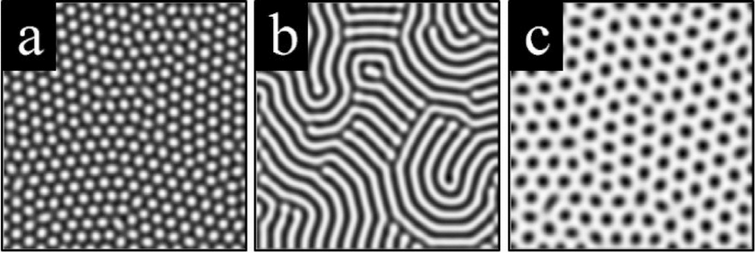
\includegraphics[scale=0.5]{01_Pre_textuais/turing2.PNG}
\end{figure}
As equações de reação-difusão são conhecidas por modelarem fenômenos químicos e biológicos, os quais, se originam da interação entre indivíduos, células ou espécies. A modelagem matemática desses mecanismos tem sido bem sucedida e vem se desenvolvendo em áreas como ecologia, embriologia (morfogênese), neurobiologia, \textcolor{red}{outros}, bem como cinéticas químicas no estado sólido. Este último tema é de interesse da ciência dos materiais computacional, uma vez que modelos matemáticos de problemas físicos tais como crescimento dendrítico (evolução cristalina), formação de precipitados em ligas metálicas e cerâmicas ou até mesmo transformação de fase por avanço de frente tornam-se possíveis.\par
Padrões espaço-temporais se apresentam em diversos âmbitos da natureza e sua descrição e compreensão ainda levantam questões importantes e básicas. Comparando com cerca de 30 anos atrás, grande progresso foi conquistado na modelagem de instabilidades, análise da dinâmica na vizinhança, formação e estabilidade de padrões, análise quantitativa experimental e numérica de padrões, e assim por diante. \par
Modelos de Reação-Difusão podem evoluir para um padrão
espacial heterogêneo e estável ao longo do tempo devido a pequenas perturbações das
concentrações das substâncias químicas em relação a um estado de equilíbrio espacial
homogêneo.\par
% Comportamentos universais de sistemas complexos próximos a instabilidades foram determinados, levando à ampla interdisciplinaridade de um campo que agora é chamado de ciência não-linear ou ciência da complexidade, e no qual conceitos iniciais de estruturas dissipativas ou sinergéticas estão profundamente enraizados.\par
% Em domínios pioneiros relacionados à hidrodinâmica ou às instabilidades químicas, as interações entre experimentalistas e teóricos, às vezes cotidianamente, têm sido fundamentais para o progresso. Todos no campo elogiam o papel desempenhado pelas interações e retornos permanentes entre estudos experimentais, numéricos e analíticos nas conquistas obtidas durante esses anos. Muitos aspectos de padrões convectivos em fluidos normais, misturas binárias ou cristais líquidos são agora entendidos e descritos neste contexto. A presença genérica de defeitos em sistemas estendidos está agora bem estabelecida e induziu novos desenvolvimentos na física de laser com grandes números de Fresnel. Por último, mas não menos importante, quase 40 anos depois de seu célebre trabalho, as estruturas de Turing foram finalmente obtidas em reatores químicos da vida real, desencadeando uma nova atividade intensa no campo dos sistemas de reação-difusão.
\textcolor{red}{Posicionar histórico, experiências, resultados, modelos, referências, etc. As teorias matemáticas...}
% \begin{figure}[H]
% \centering
% 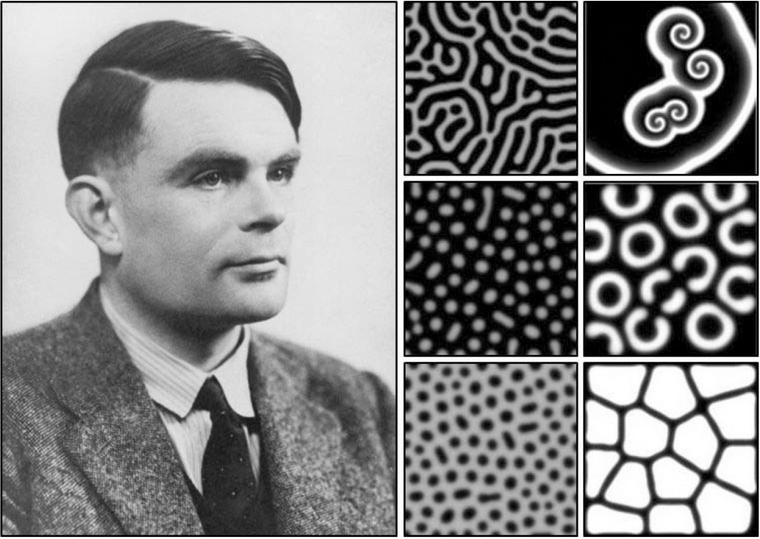
\includegraphics[scale=0.4]{01_Pre_textuais/turing1.PNG}
% \end{figure}
% \textcolor{red}{Posicionar referências}

\chapter{REVISÃO BIBLIOGRÁFICA}
\label{rev_bib}
\section{\textbf{Introdução}}
Nesta seção é apresentada a literatura utilizada, analizando-se as partes pertinentes ao trabalho realizado. Os principais tópicos de estudo foram sobre os temas de Método de Elementos Finitos, Escoamentos Multifásicos e Escoamentos Particulados em Turbomáquinas. 

\section{\textbf{Método de Elementos Finitos}}


\section{\textbf{Escoamentos Multifásicos}}
Escoamentos multifásicos são utilizados largamente na área da engenharia para uma diversidade de aplicações.
Estes ocorrem quando há o transporte de mais de uma substância em fases não miscigenadas.
Estas fases podem estar ou não no mesmo estado, subdividindo os tipos de escoamento multifásico no tipo de interação entre as fases, líquido-líquido, gás-líquido e sólido-líquido.

Dentro da engenharia mecânica pode-se verificar a grande importância destes escoamentos em casos como a extração de petróleo, onde é injetado um fluido e é captada uma mistura deste com o óleo bruto, e em trocadores de calor que possuem interação entre os fluidos.

Para os escoamentos particulados, sólido-líquido ou sólido-gás com pequenos sólidos chamados de partículas, pode-se notar sua importância até mesmo no transporte de dejetos, ná área de saneamento.%, com os chamados escoamentos de superfície livre.
Alguns exemplos na seção de mecânica incluem o transporte de vapor com condensado, formação de bolhas em bombas e sólidos precipitados.

Um dos primeiros trabalhos sobre este tipo de escoamento foi Baker et al. (1965)\cite{Baker-1965}, sobre o comportamento de escoamentos multifásicos em transportes verticais.
Estes usados bastante em trocadores de calor, como forma de melhorar sua eficiência.

%Um dos tipos de escoamentos multifásicos é o escoamento particulado, sólido-líquido ou sólido-gás, que é o foco deste trabalho.
Elghobashi et al. (1991)\cite{Elghobashi-1991} estuda o comportamento de escoamentos partículados demonstrando o efeito da turbulência na simulação de escoamentos multifásicos.

Como apresentado por Balachandar et al. (2010)\cite{Balachandar-2010}, os valores da fração de volume ocupada pela fase dispersa e a razão entre a massa da fase dispersa e a massa da fase líquida servem como indicadores do nível de interação entre as fases.
Para valores muito pequenos, o efeito dominante é do escoamento, portanto neste caso pode-se levar em conta apenas os efeitos do fluido sobre as partículas, chamado de \textit{one-way flow}.
Para casos com valores maiores, as partículas tomam um papel mais significativo no escoamento e é preciso fazer uma ligação recíproca entre os mesmos.
Portanto, recalcula-se o escoamento levando em conta os efeitos das partículas no fluido, conhecido como de \textit{two-way flow}.
E, finalmente, quando estes valores forem mais elevados a fase particulada toma um papel importante no comportamento e torna-se necessário considerar até os efeitos de outras partículas sobre cada uma delas, como colisão, aglomeração e quebra, denominado por Elghobashi et al. (1994)\cite{Elghobashi-1994} de \textit{four-way flow}.

Para a modelagem das forças atuando sobre cada partícula no escoamento foi utilizada a equação \textbf{Basset–Boussinesq–Oseen} (BBO), apresentada por Shao-Lee Soo et al. (1999)\cite{ShaoLeeSoo-1999}.
Estas equação é subdivida em várias forças atuantes, como a gravidade, arrasto, massa virtual, entre outras.
Estas equações possuem uma restrição para sua validade, podendo apenas serem aplicadas para casos com baixo número de Reynolds.


\section{\textbf{Escoamentos Particulados em Turbomáquinas}}
Dentro do ciclo de vida de uma turbomáquina, pode-se esperar um certo desgaste devido a pequenas partículas que se chocam contra as paredes durante o movimento do rotor.
Este desgate está ligado as propriedades do escoamento assim como das partículas.

Este efeito está presente até em turbinas de aeronaves, como estudado por Hussein et al. (1973)\cite{Hussein-1973}.
Este tipo de escoamento sólido-gás é verificado em locais com altos níveis de poluição.
Pode-se encontrar pequenas partículas sólidas presentes no ar ingerido por turbinas industriais e de aeronaves.
A sua presença causa um desgaste acelerado nas regiões radiais da turbina, como verificado também por Tabakoff et al. (1986)\cite{Tabakoff-1986}, que apresentou as regiões de maior colisão das partículas.
Estes trabalhos lidam diretamente com os efeitos da colisão das partículas, utilizando modelos que representam o comportamento delas após o choque.

Entrando na área de sólido-líquido, Uzol et al. (2002)\cite{Uzol-2002} fez um estudo mostranto o escoamento de uma turbomáquina utilizando partículas inseridas e um velocímetro de imagem para acompanhar seu trajeto.
Este trabalho não estuda o específicamente um escoamento particulado porém o utiliza como ferramenta para visualizar seu comportamento.

Em Ghenaiet et al. (2005)\cite{Ghenaiet-2005} é estudado com mais profundidade os efeitos dos escoamentos particulados em turbomáquinas com líquidos.
Neste caso, é estudado os efeitos da degradação causada por partículas de areia injeridas pelo escoamento na performance de uma turbomáquina axial.
Foi criado um modelo preditivo e demonstrada uma correlação entre o tamanho das partículas e a velocidade da degradação causada.

Porém a causa mais comum de erosão em impelidores de turbomáquinas trabalhando com líquidos é a cavitação.
A cavitação é a formação de bolhas de ar devido à uma queda local na pressão que logo após serem geradas implodem, gerando ondas de vibração e podendo danificar locais próximos.
A \ref{JAC-Pump} mostra os efeitos do desgaste causado pelo efeito da cavitação em uma bomba.
\begin{figure}[H]
    \centering
    \stackunder{
        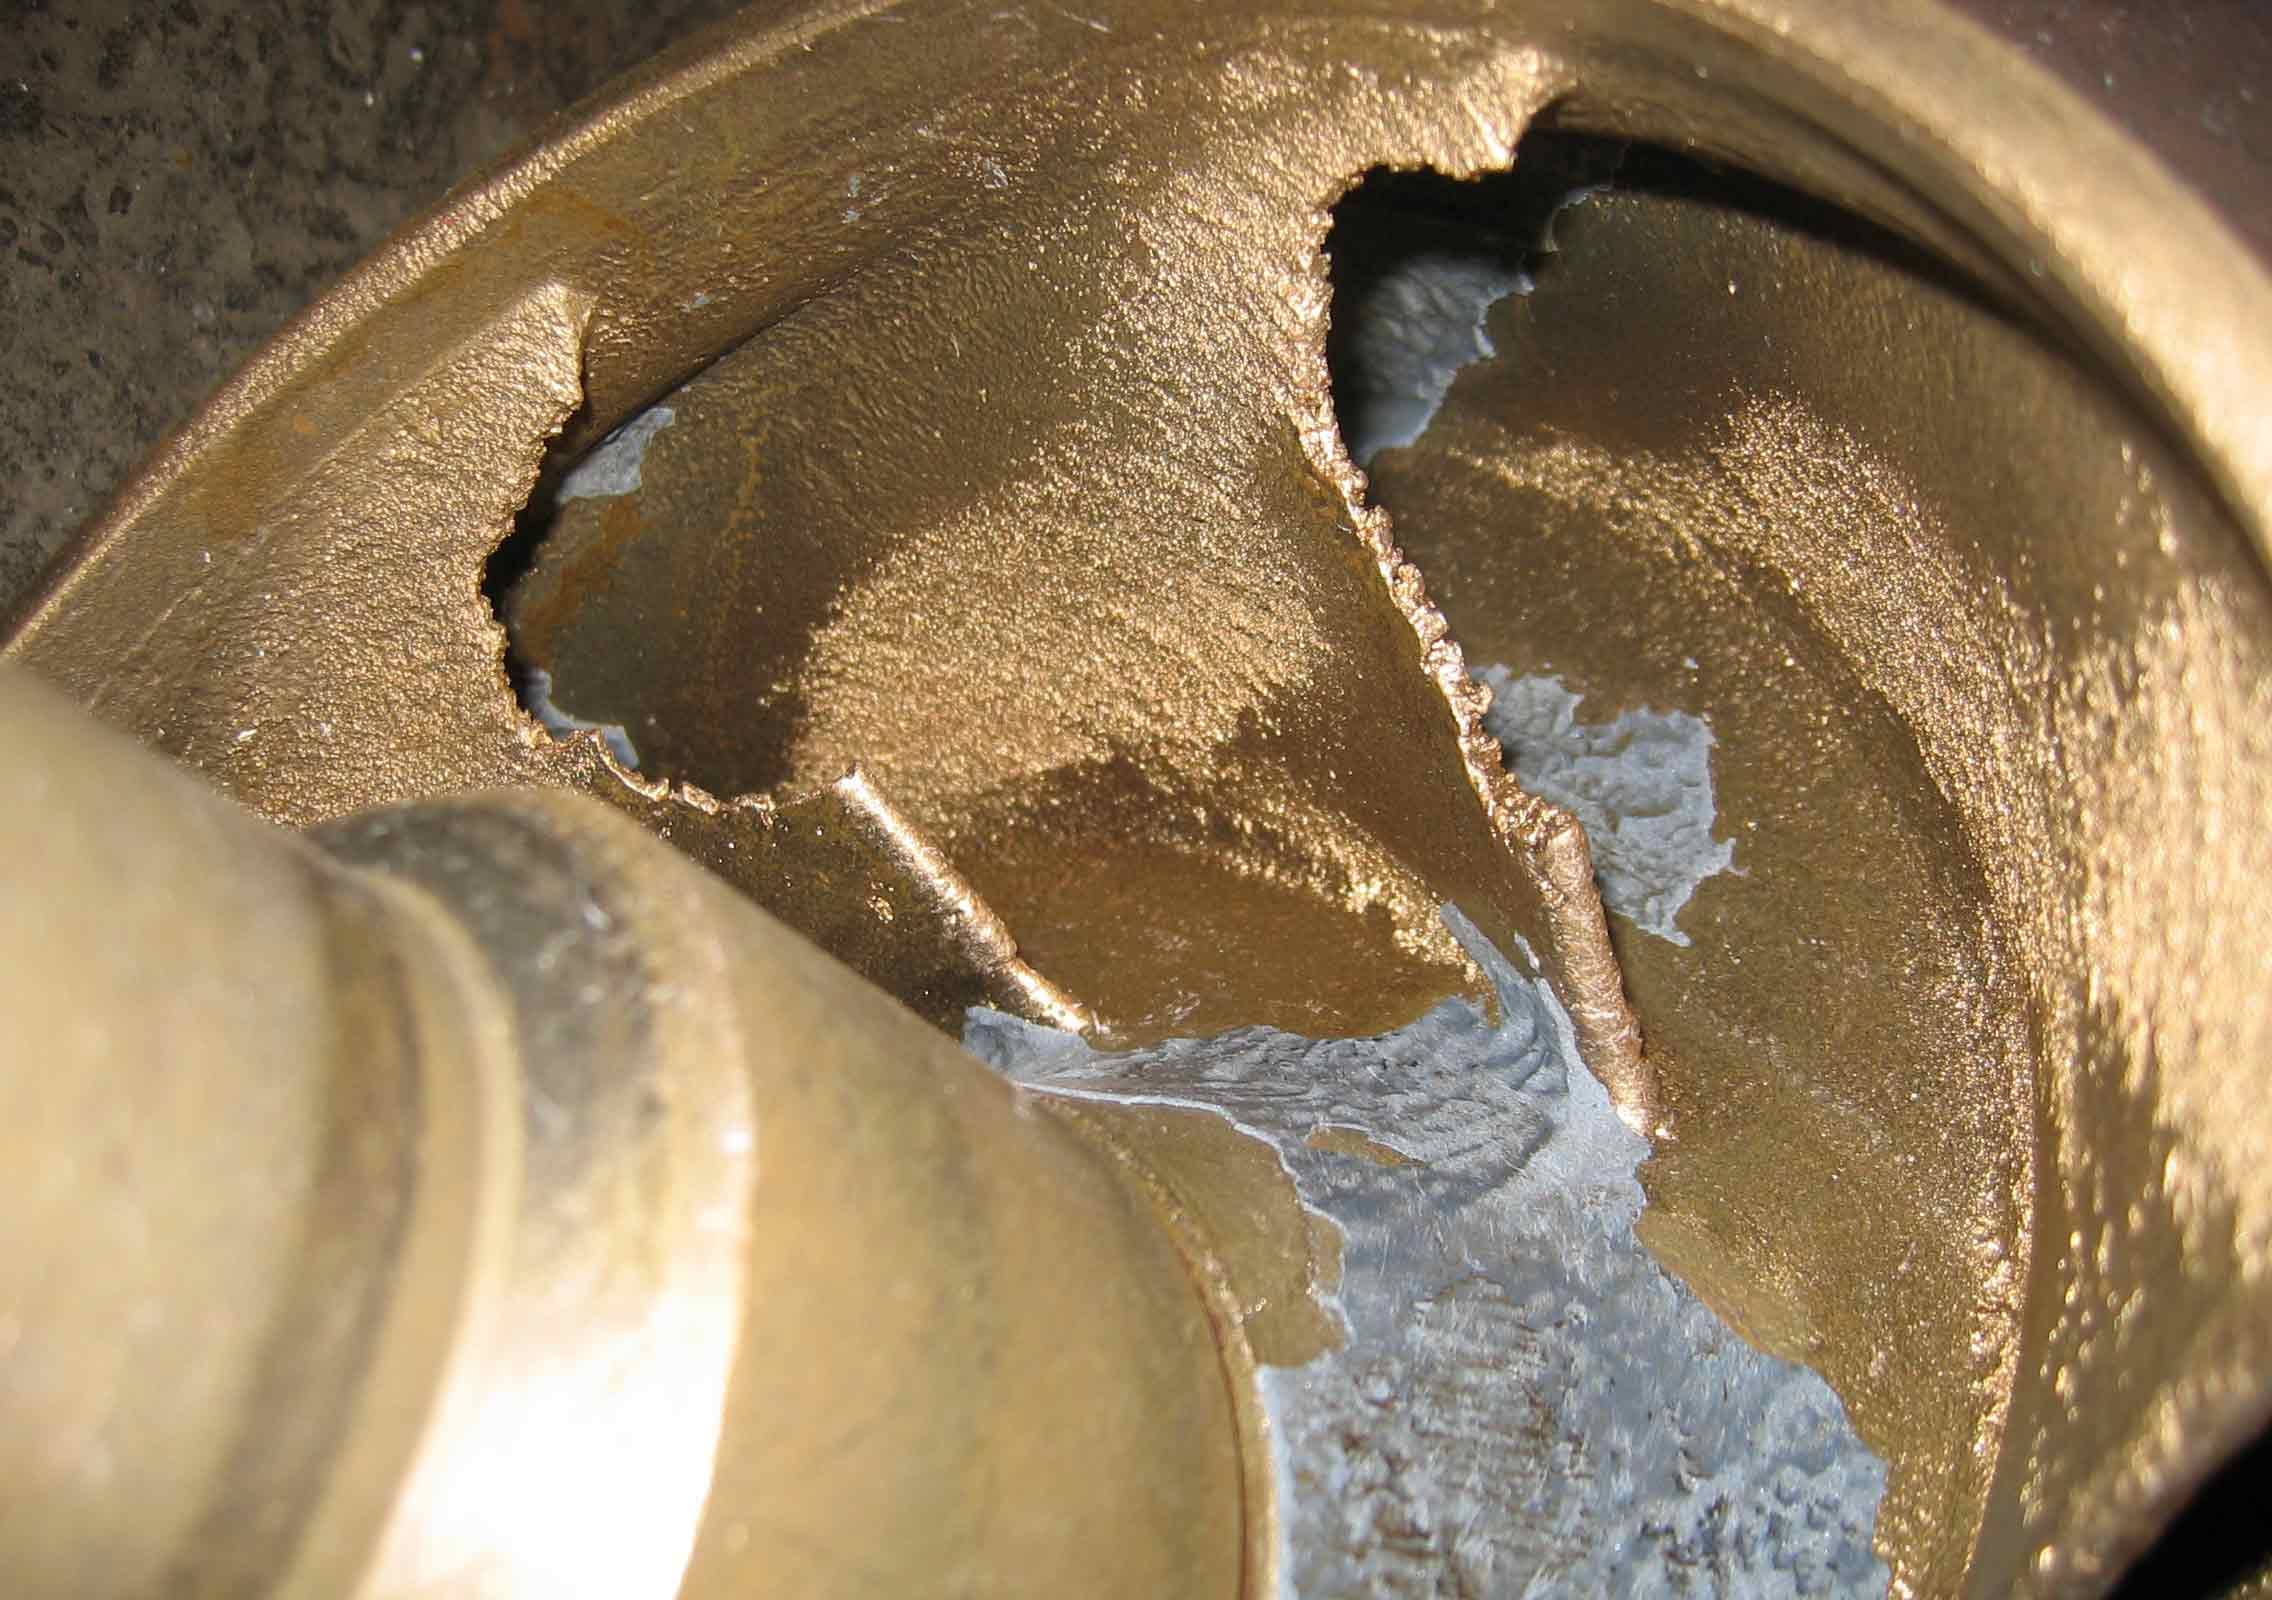
\includegraphics[width=0.6\linewidth]{figures/thermalchgo-017w2.jpg}
    } {\raggedleft \scriptsize Fonte: John Anspach Consulting\cite{JAC}.}
    \caption{Erosão em um impelidor causada pela cavitação.}
    \label{JAC-Pump}
\end{figure}

Blake et al. (1987)\cite{Blake-1987} estudou o comportamento da cavitação tomando o ponto de vista das bolhas criadas como partículas no escoamento.
Através desta interpretação, pode-se realizar simulações dos efeitos da cavitação com modelos de escoamentos particulados.

\chapter{VALIDAÇÃO DOS MODELOS}
\label{validacao}
\section{\textbf{Introdução}}
Neste capítulo serão apresentadas as validações realizadas com x exemplos conhecidos amplamente na literatura.
As validações são comparações entre os resultados numéricos obtidos pela modelagem apresentada e resultados gerados por soluções analíticas conhecidas. Elas foram separadas em três grupos que representam diferentes tipos de etapas do cálculo, desse forma espera-se demonstrar a qualidade do modelo em todas as etapas e relacionar o histórico de aprendizado e desenvolvimento do código.
São utilizadas as soluções analíticas unidimensionais dos problemas para que se possa comparar os resultados pois estas são as soluções presentes na literatura. Como os resultados são obtidos para problemas bidimensionais é preciso fazer a comparação entre resultados tomando uma seção da solução como referência, usualmente perto do meio. Essa adaptação dos dados gera uma aproximação dos resultados.

O primeiro grupo são os problemas em sólidos, que buscam confirmar a construção correta das matrizes de elementos, a aplicação apropriada dos diferentes tipos de condições de contorno e a solução de um modelo mais simples.
O segundo grupo trata dos exemplos de problemas com fluidos. 
Nesta etapa verifica-se novamente a construção das matrizes e aplicação das condições de contorno, 
porém o foco principal destes exemplos é validar o modelo e analisar as restrições de aplicabilidade.
Para o terceiro e último grupo de validações são trabalhados problemas clássicos em partículas.
São realidados testes para validar cada força trabalhando isoladamente, dessa forma facilita-se a correção pontual no modelo e pode-se comprovar com maior certeza a influência correta das forças.

Calculam-se os erros entre os resultados em cada ponto para se verificar a acurácia do modelo e sua implementação.
O erro relativo entre a solução numérica e analítica é calculado pela equação:
\begin{equation}
    er_i = \frac{(val_a)_i - (val_n)_i}{(val_a)_i}
    \label{error_eq} 
\end{equation}
Onde $(val_a)_i$ é o valor encontrado pela solução analítica e $(val_n)_i$ é o valor encontrado pela solução numérica, ambos encontrados no ponto $i$.

São calculados também a média dos erros relativos:
\begin{equation}
    er_{mean} = \frac{1}{N}\sum_{i=0}^{N} er_i
    \label{error_mean}
\end{equation}

E o desvio padrão dos erros relativos:
\begin{equation}
    er_{std} = \sqrt{\frac{1}{N}\sum_{i=0}^{N} (er_i-er_{mean})^2}
    \label{error_std} 
\end{equation}

A execução do código e computação dos resultados foram realizados em um computador de uso pessoal com as seguintes especificações:
\begin{itemize}
    \item Dell Latitude E6410 com processador Intel® Core™ i5 CPU M 520 2.40GHz com 4 núcloes e 4Gb de memória RAM.
          O sistema operacional ubuntu 16.04 LTS e compilador Python 3.5.
\end{itemize}

%---------------------------------------------------------------------------------------------------------Validação de sólidos
\section{\textbf{Validações de Problemas em Sólidos}}
%---------------------------------------------------------------------------------------------Primeiro Exemplo
\subsection{\textbf{Equação de Laplace com Condições de Contorno de Dirichlet}}
\label{sec_laplace_dir}
O problema de troca de calor em uma placa é um dos exemplos clássicos utilizados para estudar as equações de transmissão de calor em sólidos. O mais simples destes é uma barra unidimensional sem geração de calor onde a temperatura é conhecida nas extremidades.
Como a malha do código foi desenvolvida para solução de problemas bidimensionais, cria-se um problema bidimensional com condições de contorno equivalentes e extrai-se uma seção para que se possa comparar os resultados.

A equação de governo desta situação é a equação de Laplace \ref{laplace_d_perm_eq} para sólidos em estado permanente.
\begin{equation}
    \nabla^2 T = 0
    \label{laplace_d_perm_eq} 
\end{equation}
Onde T é a temperatura na placa.

E a solução analítica do problema unidimensional associado é \ref{laplace_d_sol}.
\begin{equation}
    T(x) = \dfrac{T_L-T_0}{L} x + T_0
    \label{laplace_d_sol}
\end{equation}
Onde $L$ é o comprimento da barra, $T_0$ e $T_L$ são, respectivamente, os valores da temperatura em $x=0$ e $x=L$.

Os parâmetros do problema unidimensional são definidos como:
\begin{itemize}
    \item $x\in [0,1]m$
    \item $T(0) = 0^{\circ}C$
    \item $T(1) = 1^{\circ}C$
\end{itemize}

As condições do problema bidimensional equivalente, ver \ref{laplace_d_bc}, onde a seção tomada será em $x=0.5m$, é dado por:
\begin{itemize}
    \item $x,y\in [0,1]m$
    \item $T(0,y) = 0^{\circ}C$
    \item $T(1,y) = 1^{\circ}C$
    \item $\dfrac{\partial T}{\partial n}(x,0) = 0^{\circ}C/m$
    \item $\dfrac{\partial T}{\partial n}(x,1) = 0^{\circ}C/m$
\end{itemize}

\begin{figure}[H]
    \centering
    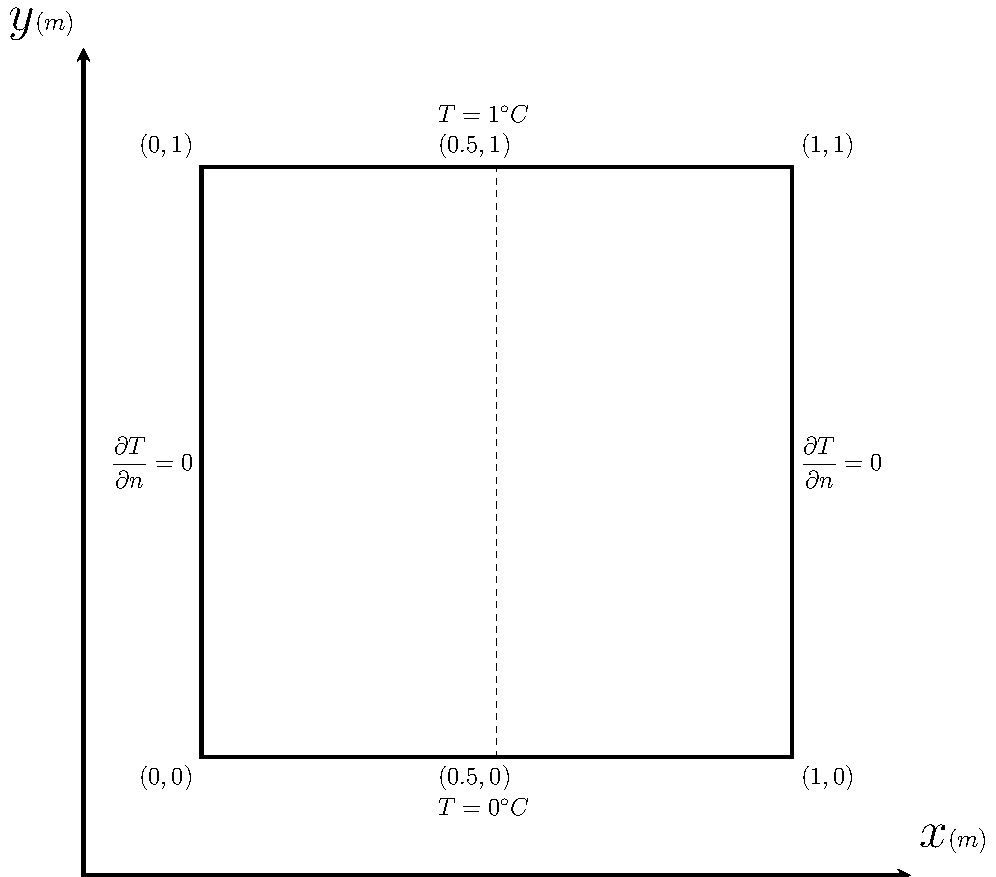
\includegraphics[width=.7\linewidth]{figures/laplace_dirichlet_boundary_conditions.pdf}
    \caption{Condições de contorno da placa para o problema de Laplace \ref{sec_laplace_dir}.}
    \label{laplace_d_bc}
\end{figure}

Para os cálculos deste exemplo foi utilizada uma malha com 768 elementos e 417 nós.
\begin{figure}[H]
    \centering
    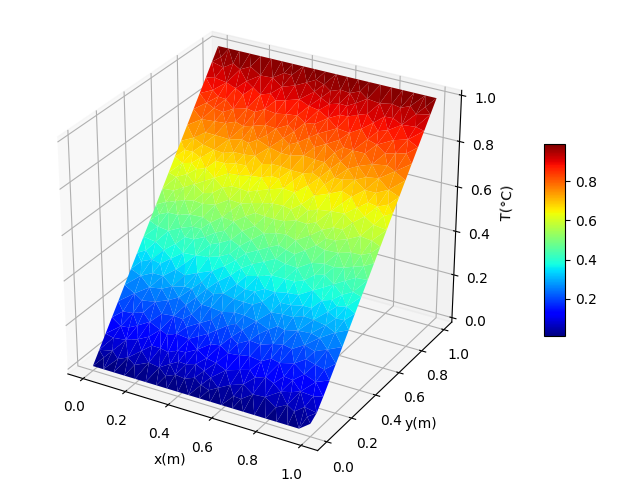
\includegraphics[width=.5\linewidth]{figures/laplace_dirichlet_permanent_3d.png}
    \caption{Distribuição de temperaturas na placa da solução permanente da equação de Laplace \ref{sec_laplace_dir}.}
    \label{laplace_d_3d}
\end{figure}

A comparação entre os resultados da solução analítica \ref{laplace_d_sol} e a solução numérica \ref{laplace_d_3d}:
\begin{figure}[H]
    \centering
    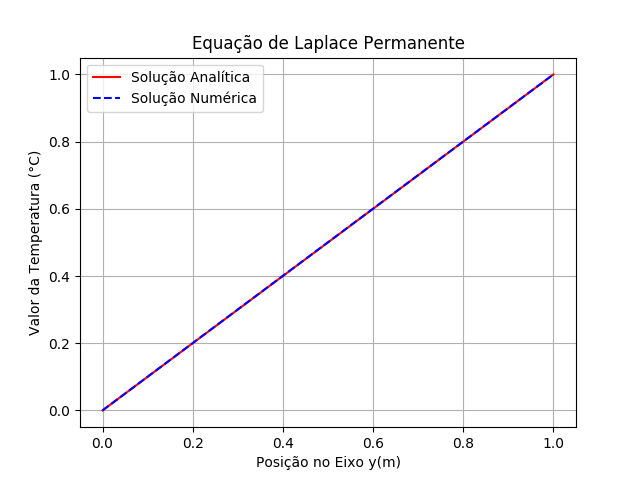
\includegraphics[width=.7\linewidth]{figures/laplace_dirichlet_permanent_comparison.png}
    \caption{Comparação de resultado das soluções númerica e analítica do caso permanente da equação de Laplace \ref{sec_laplace_dir}.}
    \label{laplace_d_perm_comp}
\end{figure}
Onde o erro relativo médio encontrado foi de $0.1136\%$ e com desvio padrão de $0.0008\%$.

Ao solucionar o mesmo problema introduzindo um termo temporal a equação de governo, pode-se verificar a evolução de comportamento da temperatura ao longo do tempo.
\begin{equation}
    \dfrac{\partial T}{\partial t} + k\nabla^2 T = 0
    \label{laplace_d_trans_eq} 
\end{equation}
Onde $k$ é o coeficiente de condutividade térmica da placa.

Porém ao longo dos passos de tempo, a solução se aproxima de um problema permanente, portanto pode-se fazer a comparação dos resultados obtidos neste exemplo com os valores da solução analítica \ref{laplace_d_sol}, tomando-se que $t\rightarrow \infty$.

Foi utilizado um critério de parada de $10^{-5}$ de variação de valores entre intervalos de tempo para obtenção dos resultados em \ref{laplace_d_trans_comp}.
As condições iniciais $t=0s$ atribuídas aos pontos sem condição de contorno foram de um valor inicial de $0^{\circ}C$.
\begin{figure}[H]
    \centering
    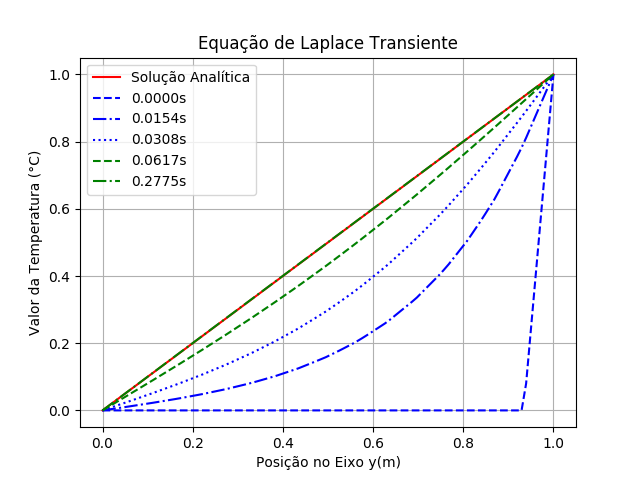
\includegraphics[width=.7\linewidth]{figures/laplace_dirichlet_transient_comparison.png}
    \caption{Comparação de resultado das soluções númerica e analítica ao longo do tempo do caso transiente da equação de Laplace \ref{sec_laplace_dir}.}
    \label{laplace_d_trans_comp}
\end{figure}
Onde o erro relativo médio encontrado foi de $0.1092\%$ e com desvio padrão de $0.0008\%$.


%---------------------------------------------------------------------------------------------Segundo Exemplo
\subsection{\textbf{Equação de Poisson com Condições de Contorno de Dirichlet}}
\label{sec_poisson_dir}
Neste problema busca-se estudar o comportamento de uma placa com geração de calor em seu domínio e temperaturas fixas nas laterais.
Novamente, para permitir a comparação de resultados, é extraída uma seção da placa para observar os resultados como um problema unidimensional.

A equação deste caso é denomidada equação de Poisson \ref{poisson_d_perm_eq}, tomada para um problema permanente, ou seja sem variação no tempo.
\begin{equation}
    -k\nabla^2 T = Q
    \label{poisson_d_perm_eq} 
\end{equation}
Onde $Q$ é a geração de calor na placa.

A solução analítica para o caso de uma barra unidimensional é descrita em \ref{poisson_d_sol}
\begin{equation}
    T(x) = \dfrac{Q}{2k}\left(-x^2 + L x\right) + \dfrac{T_L-T_0}{L} x + T_0
    \label{poisson_d_sol} 
\end{equation}

As condições do problema bidimensional, ver \ref{poisson_d_bc}, onde a seção de comparação será em $x=0.5m$, são dadas por:
\begin{itemize}
    \item $x,y\in [0,1]m$
    \item $T(0,y) = 0^{\circ}C$
    \item $T(1,y) = 0^{\circ}C$
    \item $\dfrac{\partial T}{\partial n}(x,0) = 0^{\circ}C/m$
    \item $\dfrac{\partial T}{\partial n}(x,1) = 0^{\circ}C/m$
    \item $Q(x,y) = 40W/m^2$
    \item $k = 5W/K$
\end{itemize}

\begin{figure}[H]
    \centering
    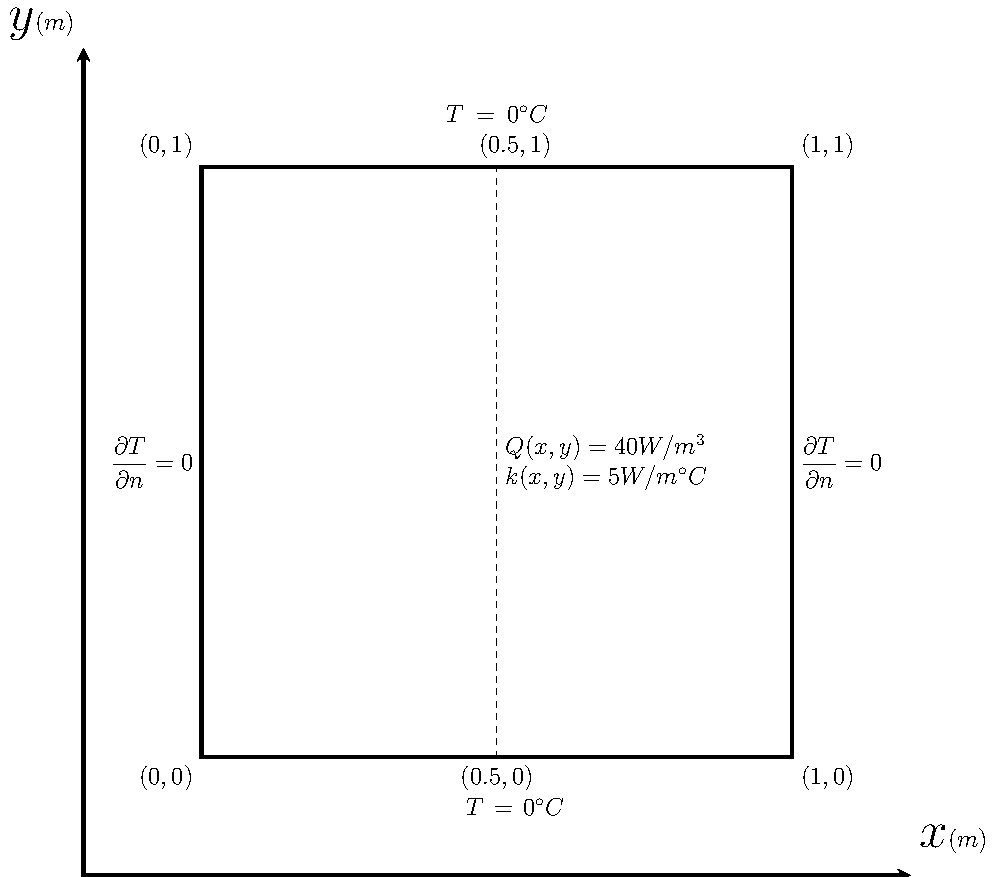
\includegraphics[width=.7\linewidth]{figures/poisson_dirichlet_boundary_conditions.pdf}
    \caption{Condições de contorno da placa para o problema de Poisson \ref{sec_poisson_dir}.}
    \label{poisson_d_bc}
\end{figure}

Novamente foi utilizada uma malha com 768 elementos e 417 nós.
\begin{figure}[H]
    \centering
    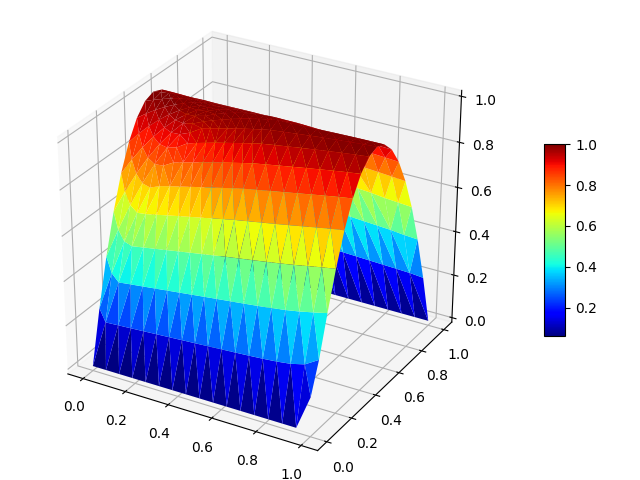
\includegraphics[width=.5\linewidth]{figures/poisson_dirichlet_permanent_3d.png}
    \caption{Distribuição de temperaturas na placa da solução do problema permanente de Poisson \ref{sec_poisson_dir}.}
    \label{poisson_d_3d}
\end{figure}

A comparação entre os resultados da solução analítica \ref{poisson_d_sol} e a solução numérica \ref{poisson_d_3d}:
\begin{figure}[H]
    \centering
    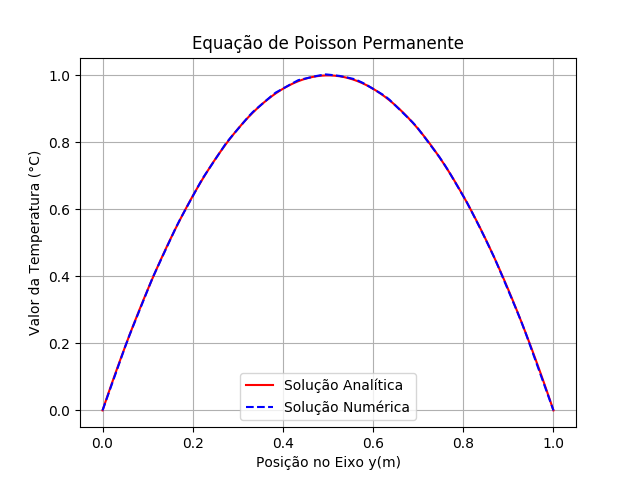
\includegraphics[width=.7\linewidth]{figures/poisson_dirichlet_permanent_comparison.png}
    \caption{Comparação de resultado das soluções númerica e analítica do problema permanete de Poisson \ref{sec_poisson_dir}.}
    \label{poisson_d_perm_comp}
\end{figure}
Onde o erro relativo médio encontrado foi de $-0.323\%$ e com desvio padrão de $0.0101\%$.

E o resultado com o termo de tempo $\dfrac{\partial T}{\partial t}$ tendendo a um estado permanente, novamente foi utilizado um critério de parada de $10^{-5}$ de diferença nos valores entre os intervalos de tempo nos resultados em \ref{poisson_d_trans_comp}.
As condições iniciais $t=0s$ atribuídas aos pontos sem condição de contorno foram de um valor inicial de $0^{\circ}C$.

\begin{figure}[H]
    \centering
    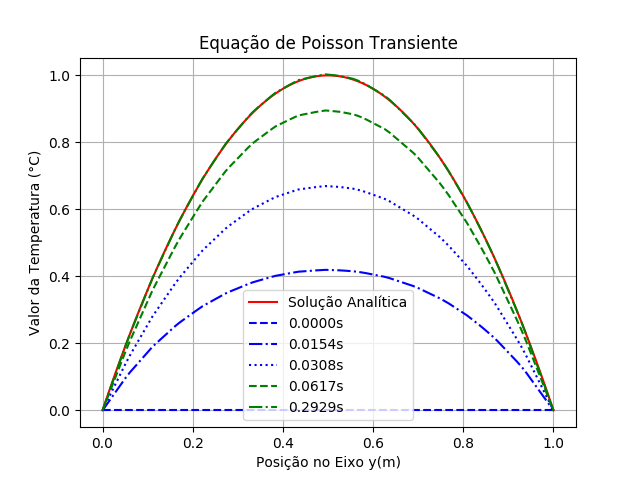
\includegraphics[width=.7\linewidth]{figures/poisson_dirichlet_transient_comparison.png}
    \caption{Comparação de resultado das soluções númerica e analítica do problema transiente de Poisson \ref{sec_poisson_dir}.}
    \label{poisson_d_trans_comp}
\end{figure}
Onde o erro relativo médio encontrado foi de $-0.325\%$ e com desvio padrão de $0.0101\%$.

%---------------------------------------------------------------------------------------------Terceiro Exemplo
\subsection{\textbf{Equação de Poisson com Condições de Contorno de Dirichlet e Neumann}}
\label{sec_poisson_neu}
Este caso foi escolhido para validar a solução de problemas com condições de contorno de Neumann.
Trata-se de uma placa com temperatura fixa em uma das paredes e no lado oposto é defido um valor para a taxa de troca de calor presente.
Toma-se uma seção da placa para observar os resultados e compará-los com um problema unidimensional de uma barra com as mesmas condições presentes.

A equação de troca térmica é novamente a equação de Poisson \ref{poisson_d_perm_eq}, com solução analítica para uma barra unidimensional \ref{poisson_n_sol}.
\begin{equation}
    T(x) = \dfrac{Q}{k}\left(\dfrac{-x^2}{2} + L x\right) + dT_L x + T_0
    \label{poisson_n_sol} 
\end{equation}
Onde $dT_L$ é o valor da taxa de troca térmica na extremidade $x=L$.

As condições do problema bidimensional, ver \ref{poisson_n_bc}, onde a seção tomada será em $x=0.5m$, são dadas por:
\begin{itemize}
    \item $x,y\in [0,1]m$
    \item $T(0,y) = 0^{\circ}C$
    \item $\dfrac{\partial T}{\partial n}(1,y) = 1^{\circ}C/m$
    \item $\dfrac{\partial T}{\partial n}(x,0) = 0^{\circ}C/m$
    \item $\dfrac{\partial T}{\partial n}(x,1) = 0^{\circ}C/m$
    \item $Q(x,y) = -7W/m^2$
    \item $k = 5W/K$
\end{itemize}

\begin{figure}[H]
    \centering
    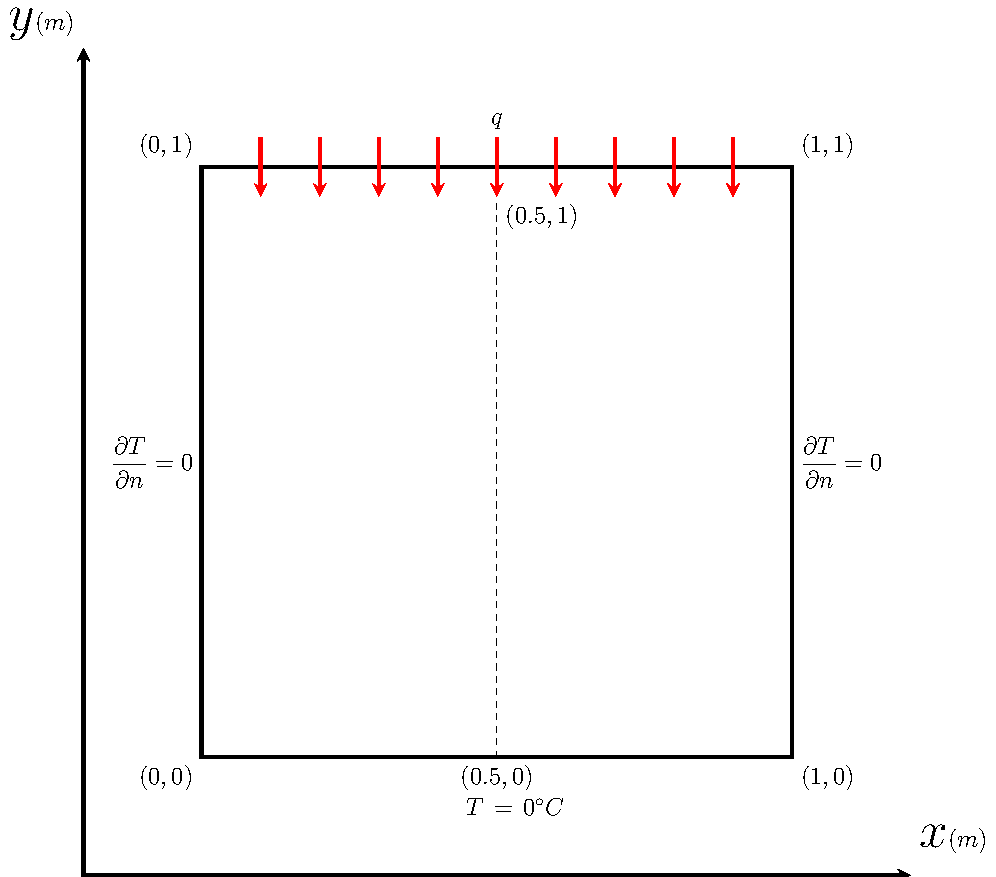
\includegraphics[width=.7\linewidth]{figures/poisson_neumann_boundary_conditions.pdf}
    \caption{Condições de contorno da placa para o problema de Poisson \ref{sec_poisson_neu}.}
    \label{poisson_n_bc}
\end{figure}

Mais uma vez foi utilizada uma malha com 768 elementos e 417 nós.
\begin{figure}[H]
    \centering
    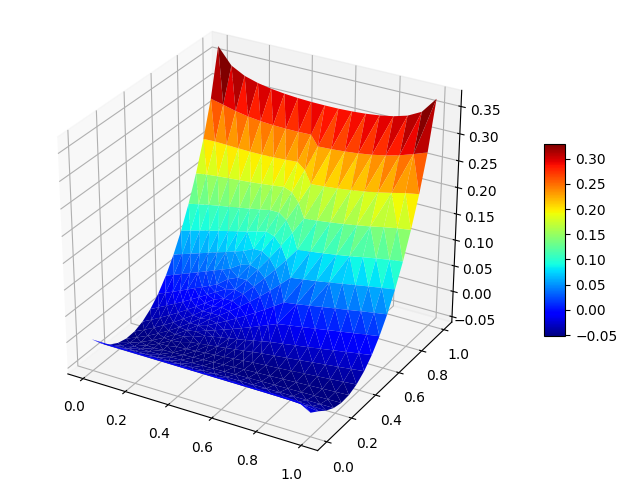
\includegraphics[width=.5\linewidth]{figures/poisson_neumann_permanent_3d.png}
    \caption{Distribuição de temperaturas na placa da solução do problema permanente de Poisson \ref{sec_poisson_neu}.}
    \label{poisson_n_3d}
\end{figure}

A comparação entre os resultados da solução analítica \ref{poisson_n_sol} e a solução numérica \ref{poisson_n_3d}:
\begin{figure}[H]
    \centering
    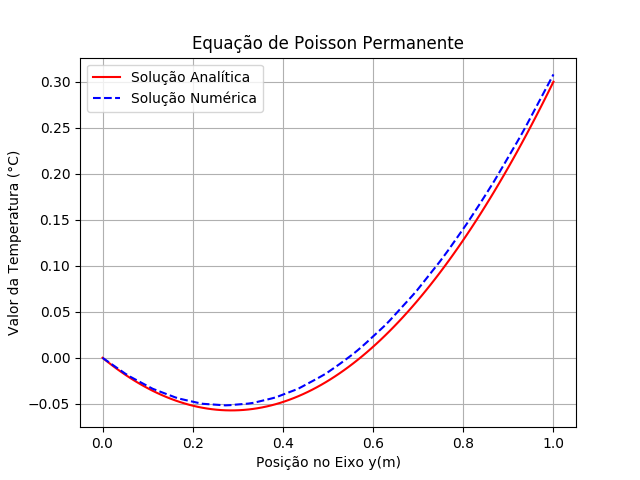
\includegraphics[width=.7\linewidth]{figures/poisson_neumann_permanent_comparison.png}
    \caption{Comparação de resultado das soluções númerica e analítica do problema permanete de Poisson \ref{sec_poisson_neu}.}
    \label{poisson_n_perm_comp}
\end{figure}
Onde o erro relativo médio encontrado foi de $-0.427\%$ e com desvio padrão de $0.8414\%$.

Para o resultado transiente foi utilizado um critério de parada de $10^{-5}$.
As condições iniciais $t=0s$ atribuídas aos pontos sem condição de contorno foram de um valor inicial de $0^{\circ}C$.

\begin{figure}[H]
    \centering
    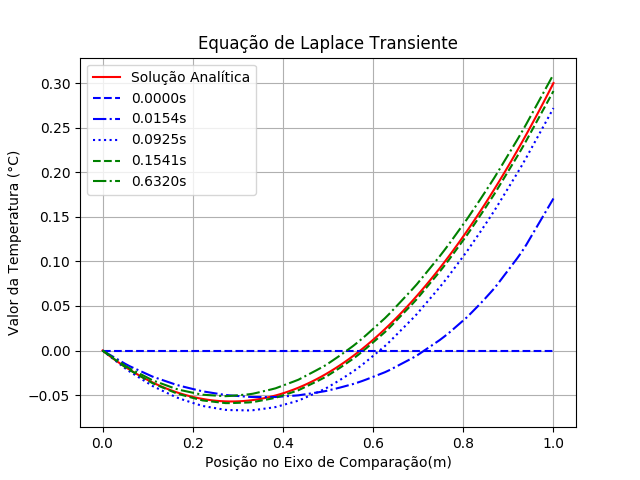
\includegraphics[width=.7\linewidth]{figures/poisson_neumann_transient_comparison.png}
    \caption{Comparação de resultado das soluções númerica e analítica do problema transiente de Poisson \ref{sec_poisson_neu}.}
    \label{poisson_n_trans_comp}
\end{figure}
Onde o erro relativo médio encontrado foi de $-0.31\%$ e com desvio padrão de $0.9205\%$.

%---------------------------------------------------------------------------------------------------------Validação de fluidos
\section{\textbf{Validações de Problemas em Fluídos}}
%---------------------------------------------------------------------------------------------Primeiro Exemplo
\subsection{\textbf{Escoamento de Hagen-Poiseuille}}
%---------------------------------------------------------------------------------------------Segundo Exemplo
\subsection{\textbf{Escoamento de Couette}}
%---------------------------------------------------------------------------------------------Terceiro Exemplo
\subsection{\textbf{Escoamento de Cavidade (\it{Lid-Driven Cavity Flow})}}


%---------------------------------------------------------------------------------------------------------Validação de partículas
\section{\textbf{Validações de Problemas em Partículas}}
%---------------------------------------------------------------------------------------------Primeiro Exemplo
\subsection{\textbf{Força Gravitacional}}

Mean Error: -3.5975243855522504e-06
Standard Error: 3.663195869072394e-06
%---------------------------------------------------------------------------------------------Segundo Exemplo
\subsection{\textbf{Força de Arrasto}}

Mean Error: 5.116557525520803e-05
Standard Error: 0.0025345030420307977
%---------------------------------------------------------------------------------------------Terceiro Exemplo
\subsection{\textbf{Força de Sustentação}}

Mean Error: 6.52554446290127e-08
Standard Error: 3.79349081853567e-08

% inserir demais capítulos aqui
% -----------------------------
% -----------------------------
% -----------------------------
% -----------------------------

\pagebreak
\addcontentsline{toc}{chapter}{\hspace{1.7cm}\bfseries CONCLUSÃO}
\noindent\textbf{CONCLUSÃO}
$\!$\\

Aqui entra sua conclusão!!

\pagebreak
\addcontentsline{toc}{chapter}{\hspace{1.7cm}\bfseries APÊNDICE A}
\setcounter{section}{0}
\setcounter{chapter}{0}%
 \renewcommand{\theequation}{A.\arabic{equation}}    
  % redefine the command that creates the equation no.
% \renewcommand{\thechapter}{\arabic{chapter}}%
\noindent\textbf{APÊNDICE A - SOLUÇÃO NUMÉRICA DA EQUAÇÃO DO CALOR BIDIMENSIONAL E VALIDAÇÃO DO CÓDIGO}
$\!$\\

% Nesse apêndice são desenvolvidas e executadas duas formas de solucionar 
% numericamente equações diferenciais parciais que possuem o termo difusivo ($\nabla^2$).

O estudo das soluções numérica e analítica de equações diferenciais parciais foi essencial para o desenvolvimento do presente trabalho. O método adotado foi o segundo esquema de Douglas \cite{DOUGLAS} (também conhecido por \textit{Stabilizing Correction}) para solução das EDP's que modelam os mecanismos de reação-difusão presentes no capítulo [4]. Como motivação, foi considerada a equação de calor bidimensional, uma vez que ela configura uma equação parabólica utilizada para modelar problemas com dependência espacial através do termo difusivo ($\nabla^2$), presente nas dinâmicas estudadas neste projeto. O desenvolvimento do código foi em \textit{python}. A equação da temperatura, com as hipóteses abaixo: 














\pagebreak
\addcontentsline{toc}{chapter}{\hspace{1.7cm}\bfseries REFERÊNCIAS}
\def\bibname{REFERÊNCIAS}
% \pagebreak
% \addcontentsline{toc}{chapter}{\hspace{1.7cm}\bfseries ANEXO A}
% \setcounter{section}{0}
\setcounter{chapter}{0}%
 \renewcommand{\theequation}{A.\arabic{equation}}    
  % redefine the command that creates the equation no.
% \renewcommand{\thechapter}{\arabic{chapter}}%
\noindent\textbf{APÊNDICE A - SOLUÇÃO NUMÉRICA DA EQUAÇÃO DO CALOR BIDIMENSIONAL E VALIDAÇÃO DO CÓDIGO}
$\!$\\

% Nesse apêndice são desenvolvidas e executadas duas formas de solucionar 
% numericamente equações diferenciais parciais que possuem o termo difusivo ($\nabla^2$).

O estudo das soluções numérica e analítica de equações diferenciais parciais foi essencial para o desenvolvimento do presente trabalho. O método adotado foi o segundo esquema de Douglas \cite{DOUGLAS} (também conhecido por \textit{Stabilizing Correction}) para solução das EDP's que modelam os mecanismos de reação-difusão presentes no capítulo [4]. Como motivação, foi considerada a equação de calor bidimensional, uma vez que ela configura uma equação parabólica utilizada para modelar problemas com dependência espacial através do termo difusivo ($\nabla^2$), presente nas dinâmicas estudadas neste projeto. O desenvolvimento do código foi em \textit{python}. A equação da temperatura, com as hipóteses abaixo: 















% abaixo segue a chamada para o arquivo [.BIB]. Utilizei o programa JABREF para montar o arquivo com minhas referências.
\nocite{*}
\bibliography{dissertacao}
\bibliographystyle{unsrt}




% \printindex    %Removi o índice remissivo para a versão oficial do trabalho.


\end{document}